\section{Bone transducer position}

The position of the \gls{bc} can ether be founded by subject test or literature search. Due to that the focus of the project is speech intelligibility of \gls{bc} and \gls{ac}, it have been chosen to do literature search on \gls{bc} positioning in stead of subject test. This have been chosen such that the test of speech intelligibility can be done more thorough due to more time for test planning and the more time of the test subject. The project can not offer money compensation to the test subject and therefore the time for testing position would than have lowered the time of speech intelligibility test. 

This section will compare earlier position test of \gls{bc} and conclude on a finite position.

\subsection{\gls{bc} position comparing}
The position of the \gls{bc} is important to ensure optimal condition for the subject test. Placement test for \gls{bc} have been research in several study and it have been shown that the condyle and mastoid position is the most favorable locations for optimal hearing \citep{cat_test}. The following \autoref{fig:condyle_mastoid} shows the  condyle and mastoid on a human.

\begin{figure}[H]
	\centering
		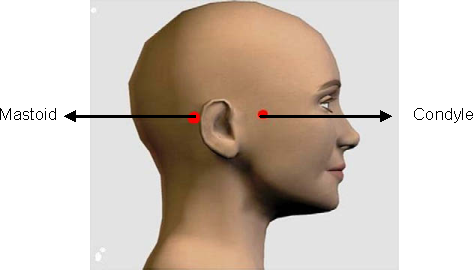
\includegraphics[width=1\textwidth]{condyle_mastoid}
		\caption{condyle and mastoid position \citep{cat_test}}
		\label{fig:condyle_mastoid}
\end{figure}

To chose the finite position of ether condyle or mastoid, the speech intelligibility and loudness perception for both position will be included in the choose. 


The article \citep{cat_test} introduce a \gls{cat} subject test, which compare  speech intelligibility with \gls{bc}. 



\gls{hint} This comparing will end out in a position of the \gls{bc}. The following \autoref{tab:test_methoed} compare the speech intelligibility for condyle and mastoid



 
\begin{table}[H]
\begin{tabularx}{\textwidth}{l X l}
\hline
\gls{cat}: & Shows that there is not statistical evidence that one of the two position of the \gls{bc} have a higher speech intelligibility over the other, but the test shows that the mean speech intelligibility score is marginal better for the mastoid. \\
\gls{hint}: & ?? \\ \hline
\end{tabularx}
\caption{Test result between condyle and mastoid for different intelligibility test and loudness test} 
\label{tab:test_methoed}
\end{table}



